\chapter{}
Manina, ou Tia Maria Angelina, dezesseis anos mais velha que eu, foi como já disse, erigida em estrela-guia da minha penosa viagem através da adolescência.
A bem da verdade, sem jamais ter postulado tal distinção, pois, por toda a minha infância, muito mais frequentemente eu recebia atenção das amigas dela, sobretudo da meiga Lygia, do que dela própria.
Quando lhe falei, muitos anos depois, sobre o importante papel que desempenhara em minha vida, reagiu com divertido assombro.
Com certeza, em razão do fato de que, assumidamente e sob mais de um aspecto, ela jamais superou a própria adolescência.
Um Peter Pan de saias foi o que ela representou para mim.

Ao mudar-se com Vovô e Vovó para uma São Paulo infinitamente menor, com ares elegantes de metrópole europeia, titia começou a realizar suas aspirações de uma vida glamourosa e cosmopolita, batizada com algumas pitadas de discreta ousadia, impossível de ser vivida na acanhada Araraquara.
Manina se pretendia um tanto boêmia, amante da boa música que se ouvia pelos barzinhos da moda, dos bons filmes, dos espetáculos teatrais, sempre que possível desfrutados na companhia de homens de classe, atraentes e muito bem vestidos, atributos que, conquanto raros, só os autorizava a candidatar-se a uma relação pouco mais que platônica, como rapidamente descobriam.
Qualquer tentativa de avançar além disso, empacava diante de um bem amarrado nó górdio: o casamento não era uma opção válida para ela e outra alternativa seria inadmissível enquanto os pais vivessem.
Ela jamais daria aos pobres velhinhos esse desgosto.
Estabelecido o impasse, o admirável era que, nesse ponto, ela conseguia sair da encrenca, na maioria das vezes, convertendo o pretendente em amigo.
Mas, é claro, só me inteirei dessas estranhas particularidades da vida amorosa da tia já mocinha, quando fui estudar em São Paulo e, aí sim, tornei-me companhia constante dela e sua confidente, até.
Para a adolescente interiorana que eu fora até esse momento, ela sempre parecera o mais acabado exemplo de feminilidade moderna, independente, irresistível.


Para melhorar o modesto salário de funcionária pública, Tia Maria Angelina dava aulas de violão.
Como suas irmãs, tinha uma bela voz e uma sensibilidade intuitiva para a boa música.
Um dia, uma das suas alunas de violão, casada com um tal Alfredo Borba, diretor artístico da gravadora Odeon, cujo elenco reunia alguns dos mais festejados ídolos musicais da época, quis apresentá-la ao marido.
Bem impressionado, o sujeito propôs a ela gravar um disco simples, de 78 rotações, uma bolacha de acetato na qual eram impressas apenas duas canções, uma de cada lado.
Manina foi às nuvens.
E ali deu início a uma carreira ainda inédita na família -- a de compositora e cantora de música popular brasileira.

\begin{figure}
\centering
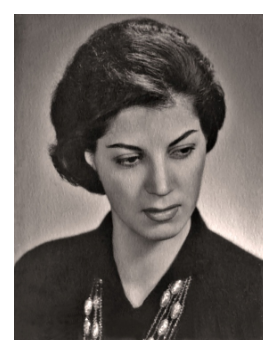
\includegraphics[width=0.7\linewidth]{14/manina-odeon.png}
\caption{Manina em foto artística para a gravadora Odeon.}
\end{figure}

Como acontecia com seus namoros, sua passagem pelo estrelato caracterizou-se pela fulguração meteórica.
Em poucos meses foi ao topo das paradas de sucesso, apresentou-se em boates famosas, em programas de rádio e televisão e, quando o sucesso começou a exigir as habituais contrapartidas em viagens, noitadas e contratos a serem cumpridos em vários lugares do país, Manina entrincheirou-se, mais uma vez, atrás de Vovó e Vovô.
Apresentando como desculpa o argumento de que já eram idosos e que ficavam apreensivos com as tentações do meio e de que ela não queria lhes causar preocupação, Deus-me-livre, etc., etc., ela voltou ao conforto seguro do anonimato.

Na carreira de funcionária pública, Manina comportou-se com diligência exemplar.
Talvez por isso não lhe faltou incentivo.
Ela chegou a ser chefe de seção na Secretaria da Fazenda e, anos depois, foi até transferida, a pedido, para a Casa Militar, no Palácio do Morumbi.
Os acréscimos de rendimento decorrentes dessas promoções e muita economia viabilizaram alguns outros sonhos que lhe eram caros: viajar para a Europa que, para ela, resumia-se praticamente à Itália, comprar um Fusquinha zero quilômetro e, mais tarde, adquirir um apartamento simples, mas bem situado, no Guarujá.

Houve uma vez em que o governo, oferecendo como estímulo a promessa de postos mais elevados e salários mais vantajosos, convidou seus funcionários a melhorar sua qualificação, facilitando-lhes o ingresso em cursos noturnos de faculdades públicas.
A maioria aderiu, entusiasmada.
Menos titia, que pretextou não poder voltar para casa tarde da noite, deixando Vovó, já então viúva, sozinha à espera.

Aos poucos, conhecendo Manina mais intimamente, comecei a me dar conta de estar na presença de uma personalidade, senão moderna e arrojada como eu julgara, pelo menos um bocado original, muito além do que supunha minha vã filosofia, para dizer o mínimo.

Uma vez um escritor, não lembro qual, declarou-se integrante da restrita parcela da humanidade capaz de ser feliz pela simples razão de ter a noção do que lhe é suficiente.
Pois, Tia Maria Angelina, estou certa, ocupou lugar de honra nessa confraria.
Foi um dos atributos que melhor a definiram e aquele que eu mais aprendi a admirar nela.
Sabia, com absoluta segurança, o que lhe convinha e não ambicionava um grama a mais.
Também não aceitava menos.
Em hipótese alguma.
Tudo quanto queria e fazia, tinha sua exata medida, não importando o que os outros dissessem.
Por isso, foi imune à inveja.
Alegrava-se genuinamente com o triunfo de parentes e amigos quando exibiam seus carrões, suas mansões ou falavam de viagens desfrutadas em \textit{resorts} deslumbrantes e restaurantes estrelados.
Porém, continuava a agradecer a Deus a felicidade proporcionada por suas próprias conquistas: o apartamentozinho do Guarujá, o seu adorado fusquinha e suas viagens econômicas para Roma.

Paradoxalmente, entretanto, gostava de ser vista como alguém familiarizado com luxo e sofisticação.
Era capaz de entrar no \textit{Copacabana Palace} e, fingindo displicência, pedir que lhe servissem um suco de laranja sob a pérgula.
Fez coisas assim muitas vezes e em variados lugares.
Sua aparência de manequim e elegância casual, na maioria das vezes, tornavam o teatrinho verossímil.
Essa mesma privilegiada aparência também lhe servia para navegar impávida em festas e \textit{vernissages}, desfilando trajes que ela se habituara a garimpar em liquidações e pontas de estoque, sem se sentir minimamente diminuída frente às joias e grifes carésimas exibidas pelas habituais frequentadoras desses ambientes.
Até gostava de alardear, com satisfação, quanto havia pago pela roupa, bolsa ou sapato, sempre que recebia elogios.


Entre suas contradições mais notórias, figurava um absoluto desinteresse por conhecer o Brasil, muito embora se declarasse patriota ardorosa, amante do samba, torcedora apaixonada do Corinthians e uma emocionada admiradora do Presidente Lula.
Contudo, sempre que chegava das suas viagens à Europa, nunca deixava de lamentar a feiura da nossa gente e das nossas cidades.
Até morrer, só abria exceção para o Rio de Janeiro.
Zona Sul, bem entendido.

Toda a independência e a quase ousadia que eu lhe atribuí ao longo da minha meninice, reduziram-se, quando a conheci melhor, à rebeldia de uma jovenzinha que, em presença do adulto, teimava em marcar posição.
Porque era engraçado como oscilava entre atitudes de aparente maturidade e objetividade frente aos problemas cotidianos e reações de insegurança e fragilidade muitas vezes infantis.
Aliás, muito embora fosse bastante alta para uma mulher da sua geração, media mais de um metro e setenta e cinco (nunca revelou quanto) e calçava número quarenta (particularidade também jamais admitida), para perplexidade das irmãs e sobrinhos, sempre teimou em comprar tudo pequeno para si: fusquinha, apartamentozinho, bicicletinha, panelinhas e sapatos invariavelmente um número menor.
E qualquer um que a presenteasse com roupas podia contar que ela haveria de sentar-se à máquina de costura para reformá-las ao seu jeito: vestidos seriam impiedosamente cortados até transformarem-se em casaquetos e mangas e golas reduzidas à metade.
Entre inconformada e zombeteira, minha mãe comentava que se alguém lhe desse um colete ela havia de dar um jeito de transformá-lo em boné! 

Enxergava-se emocionalmente como uma garotinha e quando as coisas ameaçavam ficar feias para o seu lado, refugiava-se num linguajar de criança, encolhendo-se e mostrando-se frágil demais para ser maltratada.

Contudo, encontrando brecha, nunca perdeu o gosto por desafiar.
Sempre adorou provocar os machos da família discutindo futebol ou política, assuntos que evidentemente estava bem longe de dominar.
O que não a impedia de defender seus estrábicos pontos de vista com veemência e por horas, até que só restasse aos sobrinhos e cunhados a alternativa de se dar por vencidos, para não ceder aos ímpetos de esganá-la.
Se houve uma coisa que nunca aceitou, foi ser alijada de uma discussão por ser mulher ou por não entender do assunto.


A despeito de ser totalmente egotista, duas grandes qualidades da Manina foram saber cultivar amizades e ter aversão à maledicência.
Tinha horror quase supersticioso de falar mal de quem quer que fosse.
Sua dedicação aos amigos nunca ultrapassava os limites da própria conveniência, mas era pródiga em pequenas atenções: telefonemas, lembrancinhas trazidas de viagens, convites eventuais para um cinema, uma peça de teatro, um almoço.
E mesmo quando esse ou aquele não lhe caía lá muito na simpatia, recorria ocasionalmente a uma espécie de compaixão genérica pela humanidade e convidava o infeliz para algum passeio.
Assim acontecia com a pobre Mariazinha, sua prima, uma implicante solteirona com quem se envolvia em calorosos arranca-rabos, mas que ela nunca deixou de chamar vez ou outra para sair, com pena do isolamento em que a deixavam irmãos, cunhadas e sobrinhos.

Tornava-se insuportável quando se deixava tomar de admiração por alguém, artista, político, jogador de futebol, não importa quem.
Beirava o fanatismo.
O sujeito imediatamente se revestia de todas as virtudes e que ninguém tentasse apontar no dito cujo um ou outro traço menos favorável de caráter que ela era bem capaz de avançar sobre o caluniador às unhadas.
 
Outra grande qualidade dela era saber ser grata.
Nunca esqueceu um favor recebido.
Nem desaforo, mas o sentimento causado por esse último, ela sabia disfarçar como ninguém.
Mesmo, por exemplo, quando a ofensa em questão recaia sobre o sofrido tempo vivido por João e Didi quando da falência da Mobiliadora, seu trauma maior.
Nada a feria mais fundo do que a suspeita de que houve algo de intencional no modo desastrado como Vovô conduziu o negócio.
Todavia, ainda assim, mesmo que lhe viessem lágrimas aos olhos quando ouvia insinuações de um Ópice ou outro, de que deviam ao Vovô a perda da fortuna paterna, engolia a dor.
Os primos sempre a ajudaram muito, justificava.
Mas, amargurava-se.
Porque Tia Maria Angelina idolatrava o pai, mais do que a mãe.
Morto Vovô, ela passou a vida a procurá-lo em todos os homens que conheceu.
Foi esse o segredo de polichinelo que desvendei, tão logo passei a conviver com ela.
Ela nunca quis um namorado, amante ou marido.
Ela queria um pai.
Mas tinha que ser aquele pai: o João, doce, amoroso, submisso.

A meu ver, entretanto, a coisa mais fantástica a respeito da Manina foi sua visão religiosa.
Daí lhe veio, sem dúvida, a tranquilidade e a confiança com que se permitiu fazer tudo o que bem entendeu nessa vida, sem embargo de ter sido, pela vida toda, não mais que uma reles funcionária pública, num país em que ser funcionária pública é o passaporte certo para uma vida de mediocridade sem esperança.
Manina parecia acreditar, com ingênua convicção, que tinha o Céu a seu serviço na maior parte do tempo.
Sentia-se especialmente protegida e abençoada e nem lhe passava pela cabeça perguntar-se quais eram suas credenciais para tão notória preferência.
Era assim e pronto.
A Virgem, os anjos e os santos, quando não o próprio Deus, em pessoa, livravam-na dos desastres, das doenças, dos assaltos e providenciavam o sol e o céu azul onde quer que ela chegasse.
E o pior é que, às vezes, a gente era quase obrigada a acreditar.
Pois, se houve um terremoto no país onde ela estava, Manina já ia longe, nem ficou sabendo.
Enchente, tornado, terrorismo? Só se foi depois que ela passou! Foi sempre econômica ao extremo e mesmo com seu mísero salário, após a morte da Vovó, manteve dois apartamentos, o carro, e ainda viajou várias vezes à Europa, aos Estados Unidos e à Argentina, graças às suas aplicações.
``-O meu macro'', como ela dizia, com ares de entendida.
Por influência do primo Rubens, um Ópice diretor de banco, a tia conseguiu taxas um pouco melhores para a aplicação das suas economias junto ao Banco Bradesco, nos tempos da inflação galopante dos anos 70.
Desde então, considerava-se uma privilegiada e, não importava quantos planos e sustos tivessem sacudido o país depois disso, ela nunca perdeu uma noite de sono sequer.
Tinha o seu ``macro...''

Passou por uma cirurgia séria no coração aos 68 anos e ao deixar a U.T.I, toda a queixa manifestada aos sobrinhos que, do lado de fora, esperavam por uma grave depressão pós-cirúrgica, foi a respeito do arroz ``muito empapado'' que lhe foi servido.
De resto, Deus foi bom, os médicos e enfermeiras muito atenciosos, quase não sentiu dor e ainda pôde acompanhar a novela todos os dias.

Em Cananéia, um dia, feliz porque acabara de comprar por uma ninharia uma blusa que vinha procurando há tempos, contou que entrou na igreja e, dirigindo-se ao Senhor, amorosamente censurou-o: 
{\itshape``-- Meu Deus, obrigada por ter-me feito encontrar assim tão baratinho a blusa que eu tanto queria.
Mas sabe, eu nem queria que o Senhor se preocupasse com uma coisa tão pequena! Às vezes o Senhor exagera!''}

Aos oitenta e dois anos, Tia Maria Angelina teve que refazer sua operação do coração.
A válvula instalada na cirurgia anterior esgarçou-se na aventura de uma excursão à Terra Santa, da qual havia chegado há apenas um mês.
Levei-a à emergência do hospital com pneumonia e um edema agudo de pulmão.
Um mês e uma semana depois, trouxe-a de volta para casa, de válvula nova, sã e salva.

Manina gostava de proclamar, orgulhosamente, ter poupado quantia suficiente para proporcionar a cada sobrinho, quando ela se fosse desse mundo, uma passagem de ida e volta à Europa.
E eu sempre retrucava, afirmando preferir barganhar a minha parte no tal espólio em troca da única coisa que realmente me interessava herdar dela: o seu Anjo da Guarda.

Aos noventa anos, Tia Manina já vira partir desse mundo, um a um, suas irmãs, seus amigos e experimentava a solidão e a amargura de viver sozinha em São Paulo, uma megalópolis impiedosa com os idosos.
A cada dez ou quinze dias, eu vinha de Cananéia para levá-la ao médico, fazer as compras da casa, dos remédios, atender, enfim às necessidades e problemas que a afligiam.
Não era suficiente.
Manifestando os primeiros sinais de demência senil a que se somou uma surdez irreversível, foi preciso encetar uma batalha dolorosa para derrubar o último e mais adorado bastião da sua autonomia: enviamos para Araraquara o seu fusquinha, o amado e sucateado Tatinho, que se tornara uma ameaça não só para ela própria  como para os vizinhos, transeuntes, bens e propriedades que se situassem no perímetro por onde ela circulava ao volante, olimpicamente  indiferente às buzinadas, xingamentos e expressões entre incrédulas e aterrorizadas dos circunstantes.
A essa seguiu-se outra luta, não menos cruel: acabamos por ter que enviar ela própria para Araraquara.
Paulinho, o sobrinho construtor, disponibilizara uma casa num dos seus condomínios, onde ela ficaria confortável e melhor assistida e, de lambuja, teria de volta, na garagem, completamente recuperado, o seu Tatinho!
Ainda assim, ela resistiu bravamente.
Num raro momento de lucidez, durante uma conversa na qual, pela enésima vez, eu argumentava que em Araraquara ela estaria melhor, mais segura, cercada dos sobrinhos e dos sobrinhos-netos, ela, pousando a mão sobre meu braço, interrompeu-me dizendo:
``-Teresa, eu não quis me casar, abri mão de ser mãe, de ter uma família.
Sempre soube que o preço seria terminar meus dias sozinha.''
Não obstante sua resistência, a deterioração acelerada das suas condições de saúde tornou a decisão de levá-la embora, inadiável.
Ainda viveu, como última alegria, o reencontro com seu fusquinha, novo como saído de fábrica e, mais que isso, pode dirigi-lo ainda algumas vezes nas ruas desertas do mais novo empreendimento do Paulinho, ainda em fase de implantação.
Faleceu à noite, sozinha como pressentira, numa clínica para idosos, para onde fora levada pouco tempo antes, quando já não havia como mantê-la longe de uma supervisão médica permanente.
Foi embora, deixando como lição maior para todos os que a conheceram, noventa e dois anos de uma existência que não perseguiu glória, nem fortuna, mas empenhou-se tão somente em fazer da Vida uma experiência que valeu a pena viver! 
